% Chapter 2

\chapter{Rigidity in random graphs} % Main chapter title

\label{Chapter2} % For referencing the chapter elsewhere, use \ref{Chapter1} 

\lhead{Chapter 2. \emph{Rigidity in random graphs}} % This is for the header on each page - perhaps a shortened title

%----------------------------------------------------------------------------------------

The use of the probabilistic method in discrete mathematics has become a prominent idea in the area in recent times. It provides existence proofs where objects have certain desirable properties and the construction of explicit examples is challenging. This has been just the beginning of the use of probabilistic tools within a deterministic context.

Complex topological spaces arise quite natural in a lot of scientific contexts. Probability theory implements different approaches to model those spaces; even in complex configurations, it can be possible by doing approximations, to study topological invariants. In this sense, stochastic topology can be thought as a tool for topology in the same sense as statistical mechanics is used to study a macroscopic physical system when the classical mechanics finds these systems very complicated to solve. 

Stochastic topology finds its early motivation in applied problems. Nevertheless, in recent articles it has been used to provide a deeper insight for theoretical questions. For example, with probabilistic analogs of very classical topology conjectures, like Whitehead's Asphericity Conjecture \cite[Costa, Faber 15]{Costa15}.

Probability theory can help us understand the ubiquity of certain mathematical phenomena. For example, \textit{many} simplicial complexes and posets which arise from combinatorial constructions are homotopy equivalent to a wedge of spheres, or that hiperbolicity is \textit{common} in random groups. With Probability theory we can give formal meaning to these expressions.

In this chapter we review rigid expansions in simple probabilistic models. Afterwards, we analyze the feasibility of modeling the curve graph using these proposals.

Familiarity with basic concepts in probability theory such as probability spaces, random variables, and basic theorems are assumed.

\section{Models for random graphs}

\subsection{The Radó graph}
Let $0 < p < 1$ be fixed, $\G(\N, p)$ is the probability space which consists of all graphs with vertex set $\N$, whose edges are chosen independently with probability $p$. In other words, a random graph $G \in \G(\N,p)$ is a collection $(X_{ij}) = \{ X_{ij} : 1 \leq i < j\}$ of independent $Bernoulli(p)$ r.v., where a pair $ij$ is an edge of $G$ if and only if $X_{ij} = 1$.

Erdös and Rényi proved in \cite[Erdös, Rényi 63]{RadoUnique}, that every countably infinite random graph is isomorphic to the \textbf{Radó graph}. A construction of this graph can be done using binary numbers; identify the vertices of the graph with the natural numbers and then every edge appears between vertices $x$ and $y$ in the graph (assuming $x < y$) whenever the $x$-th bit of the binary representation of $y$ is nonzero. This means, for example, that all odd-numbered vertices will be neighbors of vertex $0$, and that the larger neighbors of vertex $1$ are all vertices with numbers congruent to $2$ or $3$ mod $4$.

\begin{figure}[h!]
	\centering
	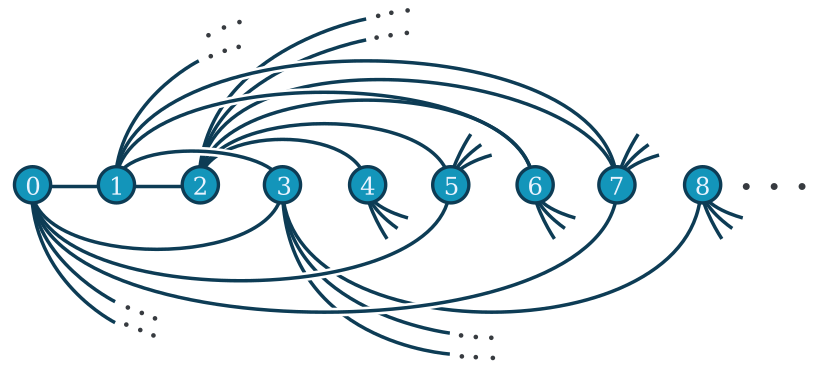
\includegraphics[scale=0.7]{Figures/Rado-graph.png}
	\caption{Binary construction of the Radó graph}
\end{figure}

\subsection{Erdös-Rényi model}
The Erdös-Rényi model for random graphs is the finite version of the Radó graph. In this model the parameter $p$ is usually taken as a function of $n$. This provides, unlike the past model, a variety of graphs when $n$ tends to infinity.

\begin{defini}
Denote by $\G(n,p)$ to the probability space formed by all the graphs of $n$ vertices and probability measure 
$$ \P\Big(G\in \G(n,p)\Big) = p^{k} (1-p)^{\binom{n}{2}-k} $$
where $k$ is the number of edges in $G$, the $\sigma$-algebra is given by the power set.
\end{defini}

Note: There is a variation of the model, where we rather choose randomly exactly $m$ edges among the $\binom{n}{2}$ possible.

We can also think this model like $\binom{n}{2}$ i.i.d. $Bernoulli(p)$ that represent the edges. From this, we can immediately get some properties of the degree of a vertex $v$.

\begin{itemize}
\item The probability that a given vertex $v$ has degree $k$ is given by
$$b(k; n-1,p) = \binom{n-1}{k} \cdot p^{k} \cdot (p-1)^{n-k-1}$$
\item The expected degree is $(n-1)\cdot p$
\item The variance of this degree is $(n-1)\cdot (1-p) \cdot p$
\end{itemize}

The degree distribution can be helpful to do optimizations in the rigid expansions algorithms. This is outlined in the next chapter.

\section{Rigid expansions}

 We will focus in the rigidity calculations for the finite case. Then, we will analyze when $n$ tends to infinite. For this, we need the calculations of the probability that the following events occur.

\begin{enumerate}
\item Given $v$ a vertex and $A_{m}$ a subset of vertices of size $m$, $v=\langle A_{m}\rangle$. Let's call $E_{m}$ to this event.
\item $A_k$ generates a rigid expansion.
\item $A_k$ generates a rigid expansion with $s$ new elements.
\end{enumerate}

For the calculations concerning the first event, take a look to following figure

\begin{figure}[h!]
	\centering
	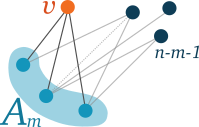
\includegraphics[scale=1]{Figures/uni.png}
	\caption{Probability of uniquely determined vertices}
\end{figure}

If $\langle A_{m} \rangle = v$, there is a edge between $v$ and every vertex in $A$, and none of the remaining $n-m-1$ vertices is also connected to every vertex in $A$, i.e.
$$\P (E_m) := \P(\langle A_{m}\rangle = v) = p^{m}(1-p^{m})^{n-m-1}$$
Using the \texttt{networkx} library in \texttt{python} we reproduce the following experiment:

\begin{cajita}
\textbf{Uniquely determined vertex experiment.} Let $n,p,m$ be fixed.
\begin{enumerate}
\item Generate an Erdös-Rényi graph $G\in \G(n,p)$ with labeled vertices.
\item Excluding the $n$-th vertex, take a random subset of vertices of size $m$.
\item Verify if this subset uniquely determine the $n$-th vertex.
\end{enumerate}
\end{cajita}

In the next chapter we explain how to generate random graphs for the first step of the experiment. To simplify the process we took, without loosing generality, the last vertex as a particular element of the experiment.

Fixing different values for $n$ and $p$ is possible to compute the empiric probability for each possible value of $m$.

\begin{figure}[h!]\label{figureExp1}
	\centering
	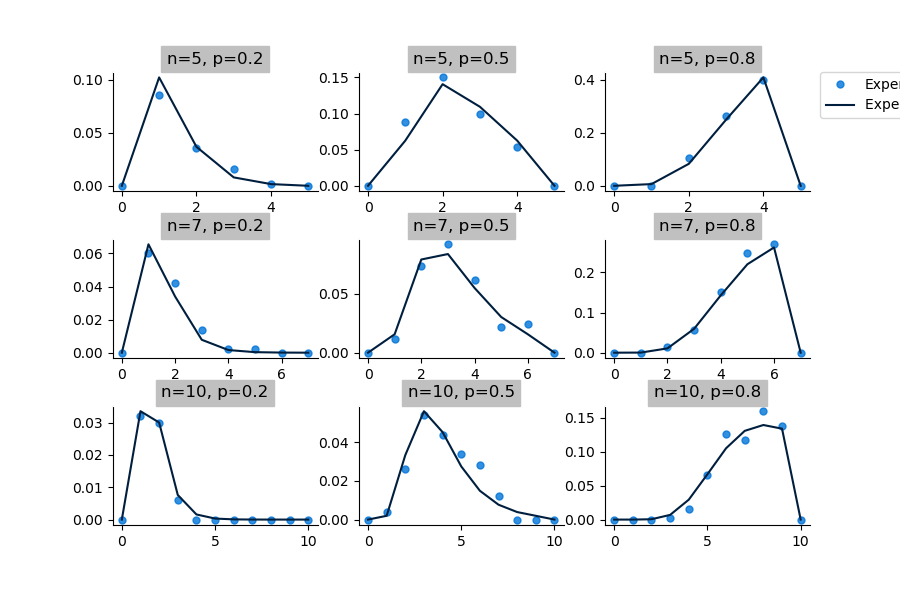
\includegraphics[scale=0.55]{Python/Figures/Uniquely-determinated-fixed-vertex.png}
	\caption{Theoretical and empirical probabilities of uniquely determined a vertex. For different values of $n$ and $p$ varying among all the possible values of $m$}
\end{figure}

For these estimations we calculated the empiric probability by repeating this experiment 500 times and counting the number of times when the $n$-th vertex was uniquely determined by the random set.

Notice that there are certain values of $m$ more \textit{effective} than others, in the sense that, depending on the parameters of the model, is more likely that a subset of certain size uniquely determine a vertex. This can be used, as described in the next chapter, to do optimizations in the simulations.

In this table appear the supremum of absolute differences between hypothesized and empirical probability $\forall m \in \{1,2, \dots n\}$ for the different values of $n$ and $p$.

\vspace{0.3cm} 
\input{Python/Txt/Uniquely-determinated-fixed-vertex-table-errors.txt}
\vspace{-0.3cm}

For the second event, if $A_k$ does not generate a rigid expansion is because none of the subsets of $A_{k}$ uniquely determined a vertex outside of it. We have:
$$\P(A_k \text{ generates a rigid expansion}) = 1 -  \prod_{m=1}^{k} (\rho_{m,k})^{\binom{k}{m}}$$
where $\rho_{m,k} = \Big(1 -  \P(E_m)\Big)^{n-k}$.

Just as before, we reproduce the following experiment:
 
\begin{cajita}
\textbf{Rigid expansion experiment}. Let $n,p,k$ be fixed.
\begin{enumerate}
\item Generate an Erdös-Rényi graph $G\in \G(n,p)$.
\item Take a random subset of vertices of size $k$.
\item Verify if this set generates a rigid expansion.
\end{enumerate}
\end{cajita}

Notice that the third step is a critical point of the experiment; we must verify among \textbf{all the possible subsets} of $A_{k}$. In the next chapter we explain the optimizations that needed to be done.

Again, we repeated this experiment 500 times and calculated the empiric probability that a random set generates a rigid expansion.

\begin{figure}[h!]\label{figureExp3}
	\centering
	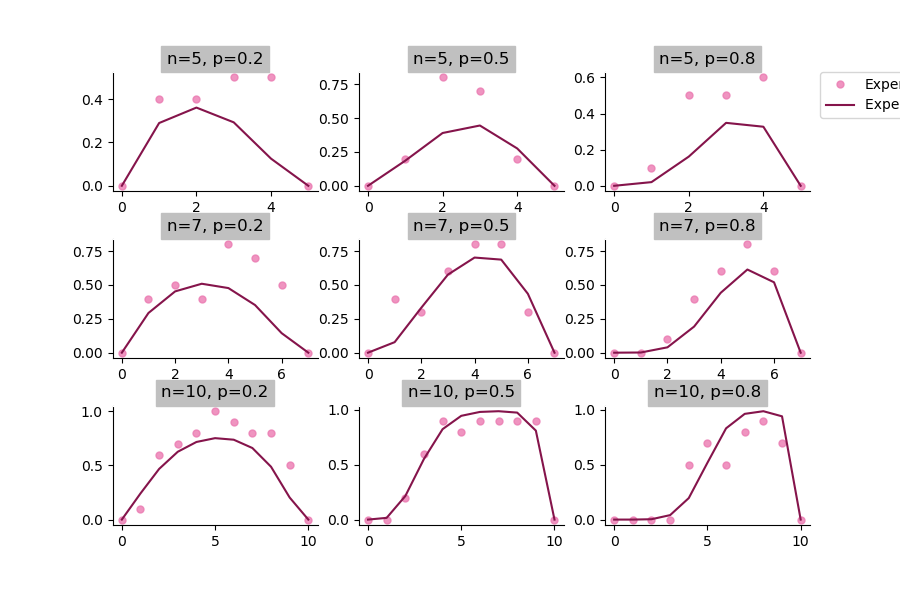
\includegraphics[scale=0.55]{Python/Figures/Expansion-probability.png}
	\caption{Theoretical and empirical probabilities of expanding $A_{k}$. For different values of $n$ and $p$ varying among all the possible values of $k$}
\end{figure}

In the following table appear the supremum of absolute differences between hypothesized and empirical probabilities $\forall k \in \{1,2, \dots n\}$ for the different values of $n$ and $p$.

\vspace{0.3cm}
\input{Python/Txt/Uniquely-determinated-fixed-vertex-table-errors.txt}
\vspace{-0.3cm}

The calculations for the last question are helpful if we want to approximate the sequence of rigid expansions of $A_{k}$ by a Markov chain. Consider $\{0,1, \dots n\}$ as the states space of the Markov chain with transition matrix given by:
$$ a_{k,k+s} = \P(A_{k} \text{ generates a rigid expansion by } s \text{ elements})$$
Notice that the deterministic process stops once a iteration fails to add new vertices. In our stochastic approximation a new $G \in \G(n,p)$ is considered for each step, hence, it is allowed to \textit{"have extra tries to expand".}

This probability calculations are more difficult to obtain. To start understanding this phenomenon we can simulate with our computational tools the following experiment:
 
\begin{cajita}
\textbf{Increase size by a rigid expansions experiment} \hfill \break
Let $n,p,k$ be fixed.
\begin{enumerate}
\item Generate an Erdös-Rényi graph $G\in \G(n,p)$.
\item Take $A_{k}$ a random set of $k$ vertices.
\item Produce the first rigid expansion from the graph spanned by $A_{k}$
\item Return the size of the expanded subgraph
\end{enumerate}
\end{cajita}

This experiment yields a random variable which depends on $n, p$ and $k$. Fixing $n$ and $p$ we obtained a sample of size 50 for every possible value of $k$. Using the resulting histogram as an empirical density function we obtain the following figure. It graphically describes the nature of the transition matrix of a sequence of rigid expansions.

\begin{figure}[h!]
	\centering
	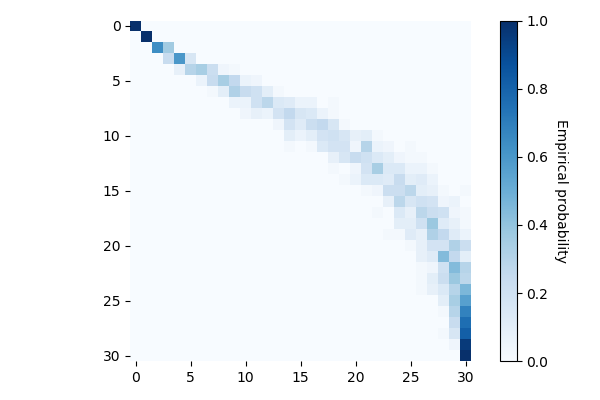
\includegraphics[scale=0.7]{Python/Figures/Transition-matrix-secuence-of-rigid-expansions.png}
	\caption{Empirical transition probability matrix}
\end{figure}

\section{Radó graph as a model for the curve graph}

In chapter one we outlined the properties of the curve graph associated to a surface, thus the proposed models should at least guarantee the following properties:

\begin{enumerate}
\item Countably infinite number of vertices
\item Connectedness
\item Locally infinite
\item Clique number $3g-3+m$
\item Infinite diameter
\end{enumerate}

The Radó graph satisfy that every finite or countably infinite graph is an induced subgraph of it \cite[Cameron 97]{theRandomGraph}. The the clique number property of $C(S)$ implies that, if $S$ is a surface of finite genus, is not possible that the Radó graph is embedded into $C(S)$. Even more, a result by Bering and Gaster \cite[Bering, Gaster 17]{beringGaster} state that the converse is also valid.

\begin{theorem}\label{beringAndGaster}
The random graph embeds into the curve graph $C(S)$ of a surface $S$ if and only if $S$ has infinite genus.
\end{theorem}

Therefore, if we want to study the curve graph of a \textbf{surface of finite genus} using the Radó graph, we have to think it as a subgraph of it. A simple approach to do it is to take a random subset of vertices of a graph $G\in \G(\N, p)$ and then consider the vertex induced subgraph. It turns out that for a.e. $G\in \G(\N, p)$ the sequence $cl(G_n)$ is almost entirely determined.

\begin{theorem}
For a.e. $G \in \G(\N,p)$ there is a constant $m_0 = m_{0}(G)$ such that if $n \geq m_o$ and $n'_{r} \leq n \leq n_{r+1}$, then $cl(G_{n}) = r$.
\end{theorem}

The theorem states that if $r$ is fixed and finite, the number of vertices must be finite as well, the proof can be find in \cite[Bollobás p.~284]{Bollobas}. Therefore, \textbf{it is not possible to obtain a curve graph by an uniform selection of vertices}.

Notice that the \textbf{clique number property is not generic} at all, unlike the others listed above, the clique number is the only property which actually depends on the genus of the surface. Therefore, is not a surprise that this property is highly restrictive in the plan of setting a generic model.

Prohibited configurations appear often in the literature, for example in \cite[Alcazar 15]{Alcazar15} they want to ensure that a random graph does not have cycles, implying that the clique number is 2. A discrete MCMC algorithm was used to sample uniformly random trees of size $n$, with the \texttt{generate algorithm}. It produces a maximal tree of any not directed graph with $n$ vertices uniformly among all the possible ones. In the appendix we summarize the results of this method, read \cite[Broder 89]{Broder89} for the full analysis.

There's a chance of finding an analog of the generate algorithm to ensure a fixed clique number, but the scope of this work is to study rigid expansions in a simple probabilistic model. In this spirit, it remains to examine the plausibility of the Erdös-Rényi model and do an asymptotic analysis.

\section{Erdös-Rényi as a model for the curve graph}

\subsection{Connectivity}
\begin{theorem}\label{connectivityER}
Let $\omega(n)$ be a function that tends to infinity arbitrarily slow as $n$ tends to infinity
\begin{itemize}
\item If $p\geq \frac{log(n)+ \omega(n)}{n}$ then 
$$\lim_{n \to \infty} \P(G \in \G(n,p) \text{ is connected}) = 1$$
\item If $p\leq \frac{log(n)- \omega(n)}{n}$ then
$$\lim_{n \to \infty} \P(G \in \G(n,p) \text{ is disconnected}) = 1$$
\end{itemize}
\end{theorem}

Here $\omega(n)$ represents the control over the convergence, in other words, the uncertainty. The theorem is just saying that in order to reduce $\omega(n)$ you must increase the size of the graph.

This theorem can be proven by first showing that for a large $n$ almost all graphs consist of a single connected component and $k$ isolated points, the theorem follows from a counting argument. The complete proof can be found in \cite[Erdös-Rényi, p.~59]{Erdos59}.
 
\subsection{Locally infinite}

To fulfill this property we need to take $p(n)$ in a way that the expected degree grows with the vertices, i.e $n p\to \infty$. Notice that the conditions for the connectivity threshold are more than enough to ensure this. The full argument is stated in the following theorem:

\begin{theorem}\label{locallyInfiniteER}
Let $G \in \G(n,p)$ and $D_{n} \sim b(k; n-1,p)$ the random variable that describes the degree of a vertex in $G$. Take $p(n)=\frac{\epsilon}{n^{a}}$ with fixed $\epsilon,a >0$ then:
\begin{itemize}
    \item If $a\geq 1$ then $\{D_{n}\} \xrightarrow[]{p} c $, where $c$ is a finite constant.
    \item If $a<1$ then $\lim\limits_{n \to \infty} \P(D_n \text{ is finite}) = 0$
\end{itemize}
\end{theorem}

\begin{proof}
When $a=1$ this is the Binomial's Poisson approximation.

For $a>1$ take $k=0$ so we have:
$$\displaystyle\lim_{n\to \infty} \P(D_n = 0) = \displaystyle\lim_{n\to \infty } \left( 1 - \frac{\epsilon}{n^a}\right)^n = \displaystyle\lim_{n\to \infty} exp\left( ln \left( 1 - \frac{\epsilon}{n^a}\right)^n\right) = \displaystyle\lim_{n\to \infty} exp\left(n \cdot ln \left( 1 - \frac{\epsilon}{n^a}\right)\right)$$
If $f(n)=  n \cdot ln \left( 1 - \frac{\epsilon}{n^a}\right)$, then $\displaystyle\lim_{n\to \infty} f(n) = \displaystyle\lim_{n\to \infty}\frac{ln \left( 1 - \frac{\epsilon}{n^a}\right)}{\frac{1}{n}}$. Using L'ôpital's rule for limits we obtain:
$$\displaystyle\lim_{n\to \infty } f(n) = 
\displaystyle\lim_{n\to \infty } \frac{\frac{1}{\left( 1 - \frac{\epsilon}{n^a}\right)}\cdot (\epsilon a n^{-a-1})}
{-1\cdot n^{-2}} = 
\displaystyle\lim_{n\to \infty } \frac{\frac{n^a}{n^{a} - \epsilon}\cdot (\epsilon a n^{-a-1}) \cdot {n^{2}}}{-1} = 
\displaystyle\lim_{n\to \infty } - \frac{\epsilon a n}{n^{a} - \epsilon} =
\displaystyle\lim_{n\to \infty } - \frac{\epsilon a}{a n^{a-1}}
$$
from here, if $a>1$ then $\displaystyle\lim_{n\to \infty } f(n) = 0$, if $a<1$ then $\displaystyle\lim_{n\to \infty } f(n) = -\infty$. So we have
$$ \displaystyle\lim_{n\to \infty} \P(D_n=0) = \begin{cases} 
\displaystyle\lim_{n\to \infty}e^{f(n)} = 1, & \mbox{if } a>1 \\ 
\displaystyle\lim_{n\to \infty}e^{f(n)} = 0, & \mbox{if } a<1 \end{cases} $$
This conclude the first part of the theorem. 

For $a<1$ and $k>0$:
\begin{center}
\begin{tabular}{ r l }
 $\displaystyle\lim_{n\to \infty } \P\Big(D_n=k\Big) =$ & $\displaystyle\lim_{n\to \infty} \binom{n}{k} \cdot \left( \frac{\epsilon}{n^a} \right)^k \cdot \left( 1-\frac{\epsilon}{n^a}\right)^{n-k}$ \\
$=$ &  $\displaystyle\lim_{n\to \infty} C_{k}\cdot n^k\cdot  \frac{\left(\frac{\epsilon}{n^a}\right)^k} {\left(\frac{n^a - \epsilon}{n^a}\right)^k} \cdot \left(1-\frac{\epsilon}{n^a}\right)^{n} $\\
$=$ &  $C_{k}\displaystyle\lim_{n\to \infty} n^k \cdot \left(\frac{1} {n^a - \epsilon}\right)^k \cdot \left(1-\frac{\epsilon}{n^a}\right)^{n} $\\
$=$ &  $C_{k} \displaystyle\lim_{n\to \infty}  n^s\cdot \left(1-\frac{\epsilon}{n^a}\right)^{n}$\\
\end{tabular}
\end{center}

where $s=k(1-a)>0$, hence $\displaystyle\lim_{n\to \infty } \P\Big(D_n=k\Big) = 0, \forall k>0$ 

\end{proof}

So, when $a<1$ we obtain the locally infinite property and this condition is always satisfied in the connectivity threshold.

The following theorem gives a complete description of the degree distribution; consider $X_{k} = X_{k} (G)$, the random variable that describes the number of vertices of degree $k$ in a graph $G$.

\begin{theorem}\label{degreeTheorem}
Let $\epsilon>0$ be fixed, $\epsilon n^{-3/2} \leq p = p(n) \leq 1 - \epsilon n^{-3/2}$, let $k = k(n)$ be a natural number and set $\lambda_{k} = \lambda_{k}(n) = \E(X_{k}) = n\cdot b(k;n - 1,p)$. Then the following assertions hold.

\begin{itemize}
\item If $\lim\limits_{n\to \infty} \lambda_{k}(n) = 0$, then $\lim\limits_{n\to \infty} \P(X_{k} = 0) = 1$. 
\item If $\lim\limits_{n\to \infty} \lambda_{k}(n) = \infty$, then $\lim\limits_{n\to \infty} \P(X_{k} > t) = 1$
for every fixed $t$.
\item If $0 < \lim\limits_{n\to \infty} \lambda_{k}(n) < \lim\limits_{n\to \infty} \lambda_{k}(n) < \infty$,
then $X_{k}$ has asymptotically Poisson distribution with mean $\lambda_{k}$: 
$$P(X_{k} = r) \sim e^{\lambda_{k}}\cdot \lambda_{k}^{r}/ r!$$
for every fixed $r$.
\end{itemize}
\end{theorem}

The $\epsilon n^{-3/2} \leq p = p(n) \leq 1 - \epsilon n^{-3/2}$ hypothesis is to rule out when we consider a loose upper bound on the expected degree of $X_ {k}$, if $pn^{2} \to \infty $ then almost every $ G \in \G (n, p) $ consist of independent edges and isolated vertices.

The first assertion comes directly from Markov's inequality and implies that if $k$ is a finite fixed number and $\lim \lambda_{k}(n) = 0$ then a.a.s. there are no vertices of degree $k$. In the second case there are an infinite number of vertices with degree $k$. In the third case we can describe explicitly the degree distribution. The complete arguments for proving this theorem can be found in \cite[Bollobás, p.~61]{Bollobas}.

\subsection{Clique number}

As outlined for the Radó graph model, the clique number is a highly restrictive property, for the Erdös Rényi model it won't be different. Let $X_r$ be the random variable that counts the number of $r-$cliques in a graph $G$, we are looking for a threshold were:
$$\lim\limits_{n \to \infty}\E(X_{r}) > 0 \text{ and } \lim\limits_{n \to \infty}\E (X_{r+1}) = 0$$
But this is not possible if $r$ is a fixed finite number. The closest we can get is stated in the following result:
\begin{theorem}\label{cliqueNumberER}
Let $r = r(n) = O(n^{1/3})$ and let $p=p(n)$, $0<p<1$, be such that
$$\binom{n}{r} p^{\binom{r}{2}} \to \infty \text{ and } \binom{n}{r+1} p^{\binom{r+1}{2}} \to 0 $$
Then a.e $G\in\G(n,p)$ has clique number $r$.
\end{theorem}

 This theorem can be proven using the calculations for $\E(X_{r})$ and a first moment argument. A full proof can be find in \cite[Bollobás, p.~290]{Bollobas}.

Given that $r(n)$ must grow along with $n$ and $r=3g-3+m$, this implies that the curve graph corresponds to a surface whether with infinite genus or with an infinite number of punctures.

\subsection{Diameter}

The diameter of a graph $G$, denoted by $diam(G)$, is the maximal distance between pairs of vertices of $G$.

If we want to model a surface of finite genus we must ensure infinite diameter, there are a number of theorems that describe the conditions under which this can be achieved \cite[Bollobás, p.~259]{Bollobas}.

Following the past result we now must guarantee that the diameter is equal to 2. The idea is to have an analogue of Bering and Gaster result (Theorem \ref{beringAndGaster}).

The next result let us see that Erdös-Rényi graphs that asymptotically approach the Radó graph, naturally satisfy the condition for the diameter.

\begin{theorem}
If $p$ is taken fixed $G(n,p)$ has diameter 2 with high probability 
\end{theorem}

\begin{proof}
Let $X_{n}$ be random variable that counts the number of vertex pairs in a graph in $\G(n,p)$ with no common neighbors. By Markov's inequality we have that
\begin{center}
\begin{tabular}{ r c l }
 $\P(X_{n} \geq 1)\leq \E(X_{n})$ & = & $\binom{n}{2} \cdot \P(\text{Two vertices doesn't have common neighbors})$ \\
 & = & $\binom{n}{2} (1-p^{2})^{n-2}$
\end{tabular}
\end{center}
where $\lim\limits_{n \to \infty}\binom{n}{2} (1-p^{2})^{n-2} = 0$
\end{proof}

Of course, we want to allow a broader type of functions to refine the previous thresholds. For this, we can use the following theorem.

\begin{theorem}\label{diameterER}
Let $d$ be a fixed integer $d$, if 
$$\frac{(pn)^{d-1}}{n} \to 0 \text{ and } \frac{(pn)^{d}}{n} \to \infty $$
then, a.a.s $G\in\G(n,p)$ has diameter $d$
\end{theorem}

The proof of this theorem is due to Klee and Larman and can be find in \cite[Klee, Larman 81]{diameters}. For $d=2$ this means we are looking that $p(n)\to 0$ and $p^2 \dot n\to \infty$, i.e $p(n)= \frac{f(n)}{n^{1/2}}$ where $f(n)\in o(n^{1/2})$ and $f(n)\to \infty$.

Using the expression for $p(n)$ in \ref{locallyInfiniteER}, we must have $a<\frac{1}{2}$ to ensure diameter 2.

\section{Conclusions}

Theorems \ref{connectivityER}, \ref{locallyInfiniteER} and \ref{diameterER} give the thresholds where each of the properties of the curve graph of infinite genus surface are satisfied. Theorem \ref{cliqueNumberER} describe the asymptotic behaviour of the clique number.

In summary, if $\epsilon, a > 0$ are fixed real number and $\omega(n)$ a function that tends to infinity arbitrary slow, we have:
\begin{enumerate}
    \item $p\geq \frac{log(n)+ \omega(n)}{n}$ $\implies$ a.a.s $G\in\G(np)$ is connected
    \item $p=\frac{\epsilon}{n^{a}}$ with $a<1$ $\implies$ a.a.s $G\in\G(np)$ is locally infinite
    \item $p=(n) = \frac{f(n)}{n^{1/2}}$ with $f(n)\in o(n^{1/2})$ and $f(n)\to \infty$, particularly if $p(n)=\frac{\epsilon}{n^{a}}$ $a<\frac{1}{2}$ $\implies$ a.a.s  $G\in\G(np)$ have diameter 2
    \item $r = r(n) = O(n^{1/3})$ with $\binom{n}{r} p^{\binom{r}{2}} \to \infty \text{ and } \binom{n}{r+1} p^{\binom{r+1}{2}} \to 0 $ $implies$ a.a.s $G\in\G(n,p)$ has clique number $r$.
\end{enumerate}

For the simplified form of $p(n) = \frac{\epsilon}{n^{a}}$ we can plot the following thresholds:

\begin{figure}[h!]
	\centering
	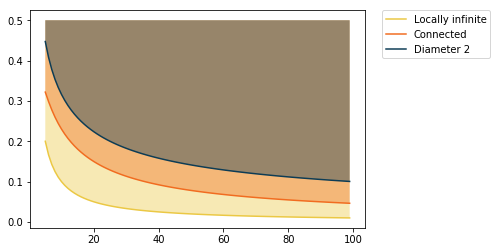
\includegraphics[scale=0.7]{Python/Figures/ER-thresholds.png}
	\caption{Thresholds for the properties of the curve complex}
\end{figure}

We can conclude that some particular properties of the random graphs, such as a fixed clique number, will be linked to the asymptotic behaviour of the vertices. Meanwhile some conditions, like diameter 2, are strong enough that other properties come along.

There is a lot of work in the study of clique complexes, for example in \cite[Khale,09]{kahle2009topology} we can find the proof of the following result:
\begin{theorem}
If $p=n^{a}$, with $a < -1/k$ or
$a > -1/2k+1$, then the k-th homology group of $X(G(n, p))$ is almost always vanishing, and if $-1/k < a < -1/(k + 1)$, then it is almost always nonvanishing
\end{theorem}

This results about homology groups can be help understand better the model for $C(S)$ asymptotically, although interpretation might not be direct.